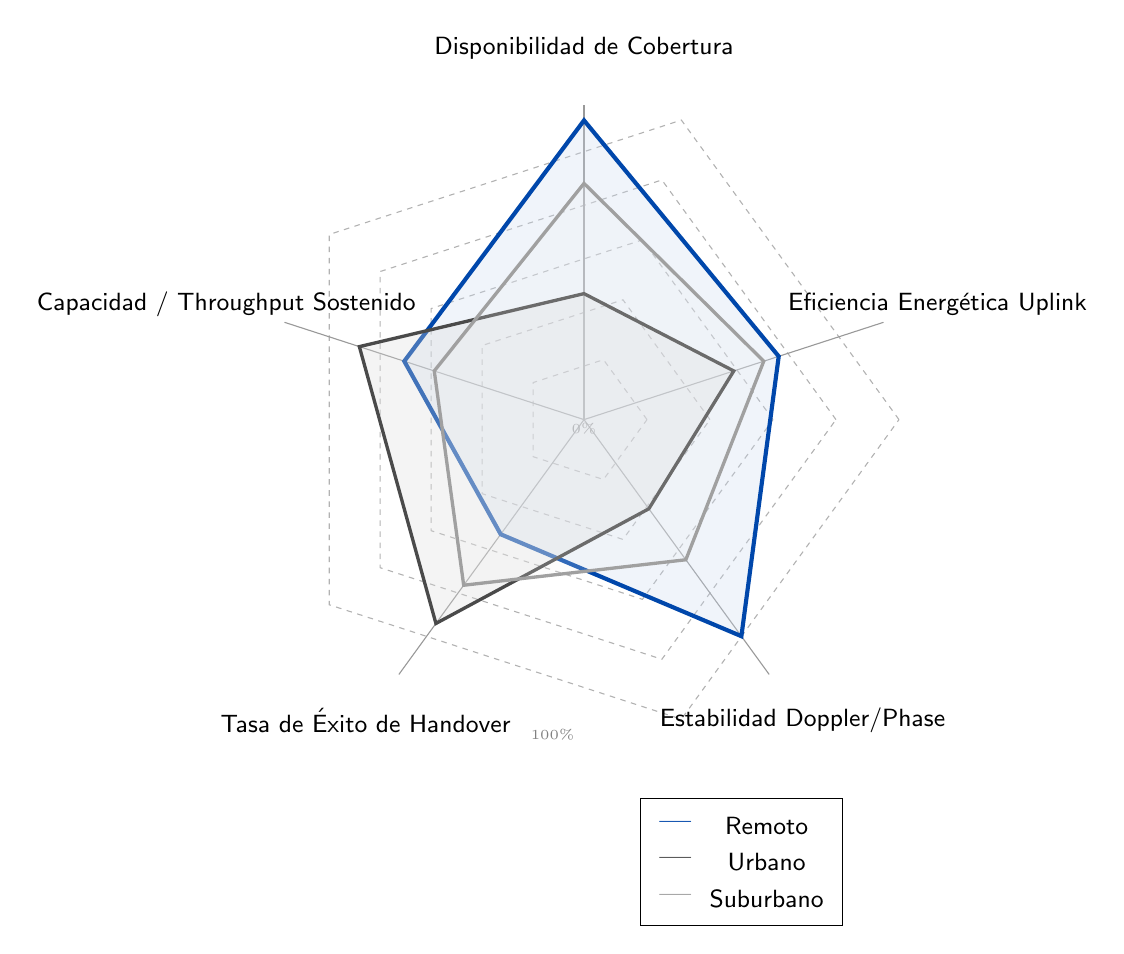
\begin{tikzpicture}[scale=4, font=\sffamily\small]
    % --- Definición Moderna de Estilos ---
    \tikzset{
        gridline/.style={dash pattern=on 2pt off 2pt, color=gray!60, thin},
        axisline/.style={color=black!40, thin}
    }
    
    % --- Dibujo de la Red Concéntrica (Grid Pentagonal) ---
    \foreach \r in {0.2, 0.4, 0.6, 0.8, 1.0} {
        \draw[gridline] (0:\r) -- (72:\r) -- (144:\r) -- (216:\r) -- (288:\r) -- cycle;
    }
    
    % --- Ejes Radiales y Etiquetas (Corregido sin la clave 'digital') ---
    \foreach \a/\label in {
        90/{Disponibilidad de Cobertura},
        18/{Eficiencia Energética Uplink},
        306/{Estabilidad Doppler/Phase},
        234/{Tasa de Éxito de Handover},
        162/{Capacidad / Throughput Sostenido}
    } {
        \draw[axisline] (0,0) -- (\a:1.0);
        \node[align=center] at (\a:1.18) {\label};
    }
    
    % Etiquetas de escala de porcentaje interno
    \node[below, gray, font=\tiny] at (90:0.02) {0\%};
    \node[left, gray, font=\tiny] at (270:1.0) {100\%};

    % --- POLÍGONO 1: REMOTO (Azul Cobalto) ---
    \definecolor{remotoblue}{HTML}{0047AB}
    \draw[color=remotoblue, line width=1.5pt, fill=remotoblue!20, fill opacity=0.3] 
        (90:0.95) -- (18:0.65) -- (306:0.85) -- (234:0.45) -- (162:0.60) -- cycle;

    % --- POLÍGONO 2: URBANO (Gris Oscuro) ---
    \definecolor{urbanogray}{HTML}{4A4A4A}
    \draw[color=urbanogray, line width=1.2pt, fill=urbanogray!20, fill opacity=0.3] 
        (90:0.40) -- (18:0.50) -- (306:0.35) -- (234:0.80) -- (162:0.75) -- cycle;

    % --- POLÍGONO 3: SUBURBANO (Gris Claro) ---
    \definecolor{suburbanogray}{HTML}{A0A0A0}
    \draw[color=suburbanogray, line width=1.2pt, fill=suburbanogray!15, fill opacity=0.2] 
        (90:0.75) -- (18:0.60) -- (306:0.55) -- (234:0.65) -- (162:0.50) -- cycle;
        
    % --- Leyenda de los Escenarios ---
    \matrix [draw, fill=white, at={(0.5,-1.2)}, anchor=north] {
        \node [color=remotoblue, font=\bfseries] {---}; & \node {Remoto}; \\
        \node [color=urbanogray, font=\bfseries] {---}; & \node {Urbano}; \\
        \node [color=suburbanogray, font=\bfseries] {---}; & \node {Suburbano}; \\
    };
\end{tikzpicture}